\section{Quantum Circuits}\newline
Ein Quantum Circuit ist ein Ausführungsplan von verschiedenen Operationen auf ein oder mehrere Qubits. Dieser Plan besteht aus Qubits, die jeweils eine horizontale Leitung mit verschiedenen Gates haben, und wird von links nach rechts gelesen. 

\begin{figure}
     \centering
     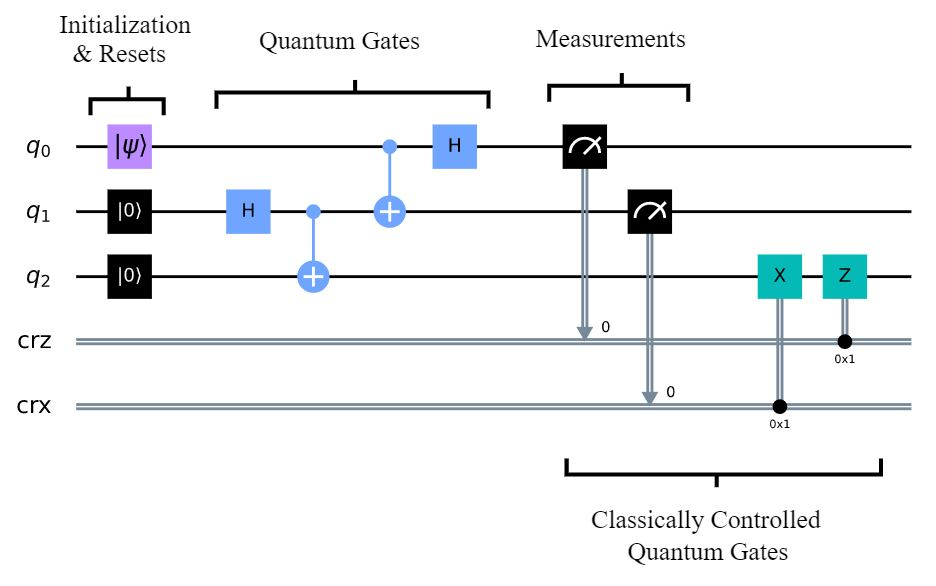
\includegraphics[width=70]{content/quantum-teleportation.JPG}

     \caption{Beispiel: Algorithmus der Quanten-Teleportation (ANIS u. a., 2021, Textbook
     ’Quantum Circuits’ - Chapter 3)}
     

\end{figure} 

\newline
Ein Quantum Circuit besteht i.d.R. aus vier verschiedenen Phasen. Die erste ist die der Initiierung, wo sich Qubits zu Beginn der Ausführung entweder standardmäßig im Zustand \(\Ket{0}\), oder nach expliziter Kennzeichnung auch in einem anderen Zustand, befinden. Danach folgen Quantum Gates, welche die Zustände der Anfangsqubits manipulieren. Anschließend werden die manipulierten Qubits gemessen und das Ergebnis als klassische Bits gespeichert. Abschließend werden unter Umständen noch von den Messergebnissen abhängige Gates ausgeführt. (ANIS u. a., 2021, Vgl. Textbook ’Quantum Circuits’ - Chapter 3)
\newline
Anzumerken ist, dass Quantum Circuits keine Loops besitzen und ausschließlich reversible bzw. unitäre Operationen durchführen. 

\newline
\newline

\subsection{Beispiel: Deutsch-Jozsa Algorithmus}
\newline
\circuit[name=circuit1,inline=true,editable=true,results=true]{content/circuit1.js}

\newline \newline
\exercise[type=multipleChoice]{
    \question{Frage: Wie wird ein Quantum Circuit gelesen?}
    \possibleAnswers{
        \item 1) Von rechts nach links.
        \item 2) Von links nach rechts.
 
    }
    \result{2}
}

\newline \newline
\exercise[type=multipleChoice]{
    \question{Frage: Was ist nicht Bestandteil eines Quantum Circuits?}
    \possibleAnswers{
        \item 1) Initiaziation & Resets
        \item 2) Quantum Gates
        \item 3) Fourier Transformation
        \item 4) Measurements
        \item 5) Clasically Controlled Quantum Gates
 
    }
    \result{3}
}
\newline \newline
\subsection{Quellen}

[ANIS u. a. 2021] Qiskit: An Open-source Framework for Quantum Computing. 2021\newline
